%%%%%%%%%%%%%%%%%%%%%%%%%%%%%%%%%%%%%%%%%
% FRI Data Science_report LaTeX Template
% Version 1.0 (28/1/2020)
% 
% Jure Demšar (jure.demsar@fri.uni-lj.si)
%
% Based on MicromouseSymp article template by:
% Mathias Legrand (legrand.mathias@gmail.com) 
% With extensive modifications by:
% Antonio Valente (antonio.luis.valente@gmail.com)
%
% License:
% CC BY-NC-SA 3.0 (http://creativecommons.org/licenses/by-nc-sa/3.0/)
%
%%%%%%%%%%%%%%%%%%%%%%%%%%%%%%%%%%%%%%%%%

%----------------------------------------------------------------------------------------
%	PACKAGES AND OTHER DOCUMENT CONFIGURATIONS
%----------------------------------------------------------------------------------------
\documentclass[fleqn,moreauthors,10pt]{ds_report}
\usepackage[english]{babel}

\graphicspath{{fig/}}

%----------------------------------------------------------------------------------------
%	ARTICLE INFORMATION
%----------------------------------------------------------------------------------------

% Header
\JournalInfo{FRI Natural language processing course 2025}

% Interim or final report
\Archive{Project report} 
%\Archive{Final report} 

% Article title
\PaperTitle{Automatic generation of Slovenian traffic news for RTV Slovenija} 

% Authors (student competitors) and their info
\Authors{Marjan Stojchevski, Gal Šubic, and Aleksander Osvald}

% Advisors
\affiliation{\textit{Advisors: Slavko Žitnik}}

% Keywords
\Keywords{Keyword1, Keyword2, Keyword3 ...}
\newcommand{\keywordname}{Keywords}

%----------------------------------------------------------------------------------------
%	ABSTRACT
%----------------------------------------------------------------------------------------

\Abstract{
%The abstract goes here.
}

%----------------------------------------------------------------------------------------

\begin{document}

% Makes all text pages the same height
\flushbottom 

% Print the title and abstract box
\maketitle 

% Removes page numbering from the first page
\thispagestyle{empty} 

%----------------------------------------------------------------------------------------
%	ARTICLE CONTENTS
%----------------------------------------------------------------------------------------

\section*{Introduction}
% ------- INSTRUCTIONS --------
% In the Introduction section you should write about the relevance of your work (what is the purpose of the project, what will we solve) and about \textbf{related work} (what solutions for the problem already exist). Where appropriate, reference scientific work conducted by other researchers. 
% The abbreviation et al., which in latin means and others, is used when there are more than two authors of the work we are citing.
% If there are two authors (or if there is a single author) we just write down their surnames. 

The goal of this project is to automate the writing of Slovenian radio traffic reports from traffic information. These are currently being manually written by students and since this is a repetitive task that involves processing large amounts of data, we want to automate it using increasingly popular large language models (LLM's).
Reports generated this ways should not only be factually correct and concise, but should also stick to established report form and naming conventions. Generating text in Slovene also poses a challenge, as most LLM's and their evaluation methods are better suited for English language.

\subsection*{Related works}
G. Taghizadeh \cite{llmReporting} talks about how how multi agent LLMs are affecting reporting, J. Pereira et al. adresses the broader field of news \cite{pereira2024generation}.

\subsection*{Dataset}
The data for the project was already provided. It consists of three main parts: input data, output data (traffic reports) and rules and guidelines, which have to be taken into account when making reports. The input was collected from 2022 to 2024 from \url{promet.si} and the output consists of reports from RTV SLO. 

The input data contains different categories of traffic information such as accidents, traffic jams, road work, weather related information and vehicle restrictions.
The output data contains structured reports which are in accordance with rules and guidelines. They are further split into urgent reports (Nujna prometna informacija), which are broadcast when needed, and regular reports (Prometna informacija) which are broadcast at regular intervals every half hour.

The rules and guidelines are meant for human writers to correctly structure the report and use the proper terms and names. They include traffic information word structure, traffic event hierarchy, road and highway informal names, which are better understandable and more commonly used, and other relevant information.


\subsection*{Initial ideas}
Although such a task could - to a degree - be accomplished using prompt engeneereng, it proves difficult to generate a report that accurately describes cause and effect, while sticking to a desired format.
Instead in our approach, we evaluate the base models LLaMA and SambaLingo-Slovenian-Base, which we fine-tune for the task using LoRA Parameter Efficient Fine-Tuning (PEFT). 

While human evaluation would assess fluency and correctness of generated reports best, it is not an option for this assignment. We could use BERTScore \cite{bert-score} as an automatic measure of similarity between our models output and RTV SLO reports. BERTScore is a language-independent evaluation metric that measures the similarity between generated and reference text using contextual embeddings from transformer models. Alternative measures include the likes of BLEU, ROUGE, METEOR, but these are not the most suitable for Slovene due to its flexible word order and rich word morphology.
A possible alternative is evaluation using other LLMs like GPT-4-turbo (ChatGPT) which understands Slovene language to compare the human-written and our machine-generated report. This approach could be especially useful for determining wheter the generated reports are in accordance with the reporting and naming guidelines.
Lastly we could use some naive methods, such as comparing certain keywords that would have to appear in the report, such as names of locations and highways.
For the test dataset we can use the last 6 months (equating to roughly 20\%) of our dataset for evaluation or we can sample the reports evenly through time.

%------------------------------------------------

\section*{Methods}
% INSTRUCTIONS
% Use the Methods section to describe what you did and how you did it -- in what way did you prepare the data, what algorithms did you use, how did you test various solutions ... Provide all the required details for a reproduction of your work.

\iffalse
\LaTeX examples of some common elements that you will probably need when writing the report (e.g. figures, equations, lists, code examples ...).

\subsection*{Equations}

You can write equations inline, e.g. $\cos\pi=-1$, $E = m \cdot c^2$ and $\alpha$, or you can include them as separate objects. The Bayes’s rule is stated mathematically as:

\begin{equation}
	P(A|B) = \frac{P(B|A)P(A)}{P(B)},
	\label{eq:bayes}
\end{equation}

where $A$ and $B$ are some events. You can also reference it -- the equation \ref{eq:bayes} describes the Bayes's rule.

\subsection*{Lists}

We can insert numbered and bullet lists:

% the [noitemsep] option makes the list more compact
\begin{enumerate}[noitemsep] 
	\item First item in the list.
	\item Second item in the list.
	\item Third item in the list.
\end{enumerate}

\begin{itemize}[noitemsep] 
	\item First item in the list.
	\item Second item in the list.
	\item Third item in the list.
\end{itemize}

We can use the description environment to define or describe key terms and phrases.

\begin{description}
	\item[Word] What is a word?.
	\item[Concept] What is a concept?
	\item[Idea] What is an idea?
\end{description}

\subsection*{Figures}

You can insert figures that span over the whole page, or over just a single column. The first one, \figurename~\ref{fig:column}, is an example of a figure that spans only across one of the two columns in the report.

\begin{figure}[ht]\centering
	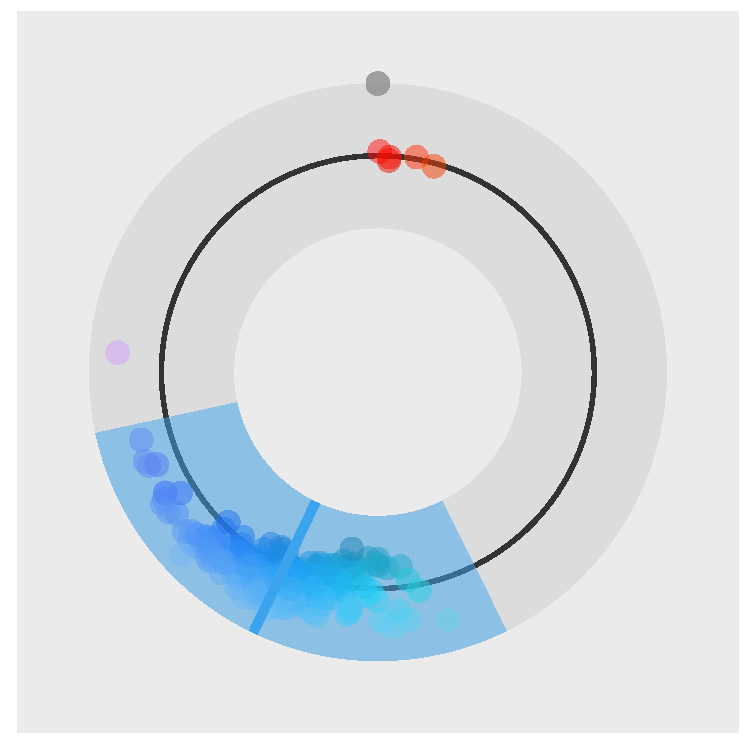
\includegraphics[width=\linewidth]{single_column.pdf}
	\caption{\textbf{A random visualization.} This is an example of a figure that spans only across one of the two columns.}
	\label{fig:column}
\end{figure}

On the other hand, \figurename~\ref{fig:whole} is an example of a figure that spans across the whole page (across both columns) of the report.

% \begin{figure*} makes the figure take up the entire width of the page
\begin{figure*}[ht]\centering 
	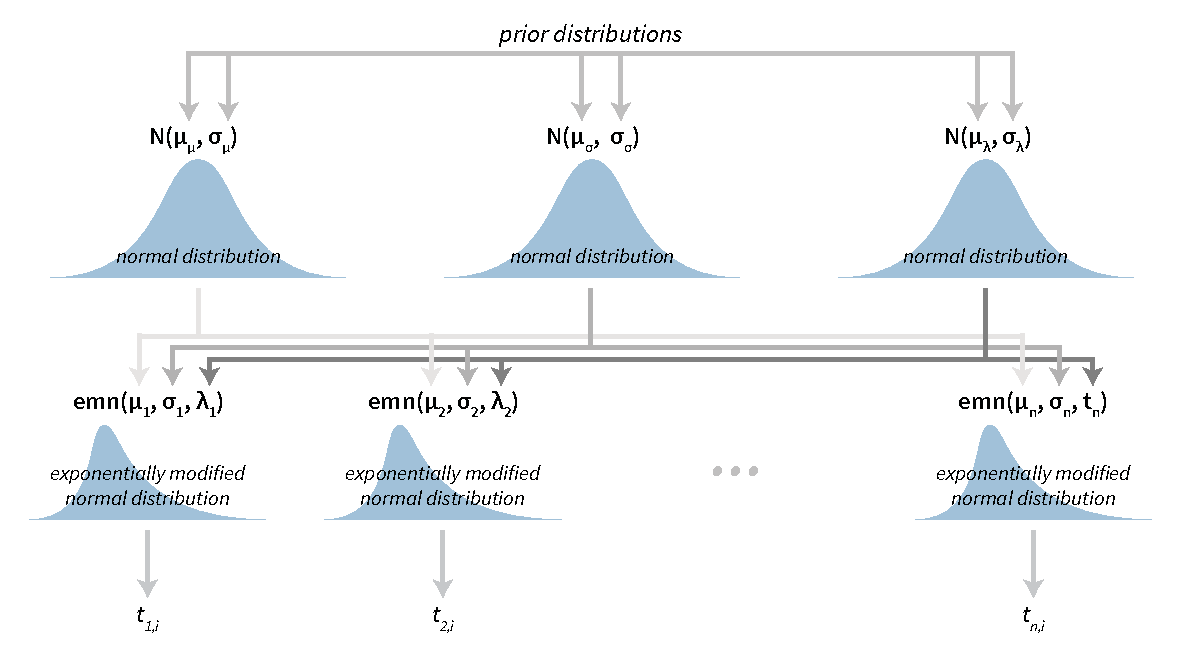
\includegraphics[width=\linewidth]{whole_page.pdf}
	\caption{\textbf{Visualization of a Bayesian hierarchical model.} This is an example of a figure that spans the whole width of the report.}
	\label{fig:whole}
\end{figure*}

\subsection*{Tables}

Use the table environment to insert tables.

\begin{table}[hbt]
	\caption{Table of grades.}
	\centering
	\begin{tabular}{l l | r}
		\toprule
		\multicolumn{2}{c}{Name} \\
		\cmidrule(r){1-2}
		First name & Last Name & Grade \\
		\midrule
		John & Doe & $7.5$ \\
		Jane & Doe & $10$ \\
		Mike & Smith & $8$ \\
		\bottomrule
	\end{tabular}
	\label{tab:label}
\end{table}

\subsection*{Code examples}

You can also insert short code examples. You can specify them manually, or insert a whole file with code. Please avoid inserting long code snippets, advisors will have access to your repositories and can take a look at your code there. If necessary, you can use this technique to insert code (or pseudo code) of short algorithms that are crucial for the understanding of the manuscript.

\lstset{language=Python}
\lstset{caption={Insert code directly from a file.}}
\lstset{label={lst:code_file}}
\lstinputlisting[language=Python]{code/example.py}

\lstset{language=R}
\lstset{caption={Write the code you want to insert.}}
\lstset{label={lst:code_direct}}
\begin{lstlisting}
import(dplyr)
import(ggplot)

ggplot(diamonds,
	   aes(x=carat, y=price, color=cut)) +
  geom_point() +
  geom_smooth()
\end{lstlisting}
\fi

%------------------------------------------------

\section*{Results}
% INSTRUCTIONS
% Use the results section to present the final results of your work. Present the results in a objective and scientific fashion. Use visualisations to convey your results in a clear and efficient manner. When comparing results between various techniques use appropriate statistical methodology.

%------------------------------------------------

\section*{Discussion}
% INSTRUCTIONS
% Use the Discussion section to objectively evaluate your work, do not just put praise on everything you did, be critical and exposes flaws and weaknesses of your solution. You can also explain what you would do differently if you would be able to start again and what upgrades could be done on the project in the future.


%------------------------------------------------

\section*{Acknowledgments}
% INSTRUCTIONS
% Here you can thank other persons (advisors, colleagues ...) that contributed to the successful completion of your project.


%----------------------------------------------------------------------------------------
%	REFERENCE LIST
%----------------------------------------------------------------------------------------
\bibliographystyle{unsrt}
\bibliography{report}


\end{document}